% !TEX root = ../seapp-manual.tex

% Chapter 0 - Introduction

\chapter{Intoduction}
\label{ch:intro}

\texttt{SEA++} is an attack simulator based on \texttt{INET/OMNeT++} network simulator. It allows the reproduction of effects of successfull attacks and the quantitative evaluation of their impact. \texttt{SEA++} is a complete simulation tool which helps the user to evaluate the impact of cyber/physical attacks.  It has to be clarified that \texttt{SEA++} does not find new attacks neither evaluate the feasibility of them. The user does not need to implement the adversary model as the actual way of attack's execution is out of scope of \texttt{SEA++}. The user only describes the attack scenario and evaluates the impact of the successfull attack. \\

\texttt{SEA++} consists of 3 basic components; \texttt{(i)} the high level \emph{Attack Description Language (ADL)}, \texttt{(ii)} the \emph{Attack Interpreter} and \texttt{(iii)} the \emph{Engine}. The user describes the attack scenarios using the ADL. The interpreter converts the attack file \texttt{.adl} to the Attack Configuration File \texttt{.xml}, which is given as input to the Engine. The Engine injects the atomic events at runtime during the network simulator based on the Attack Configuration File. The two basic components of the Engine are the \emph{Local Filter} and the \emph{Global Filter}. The Local Filter is the component which communicates with all the layers of the OSI stack of a node being able to intercept, inject, modify or drop the packets. The Local Filters of all the nodes within the network communicate with the Global Filter which represents an external entity in the network. The two components handle the 3 different types of attacks; \emph{physical}, \emph{conditional} and \emph{unconiditonal} attacks. The Local Filter is responsible to perform the physical and the conditional attacks based on the ADL primitives, while the Global Filter is responsible for the unconditional attacks. \\

\begin{figure}[h]
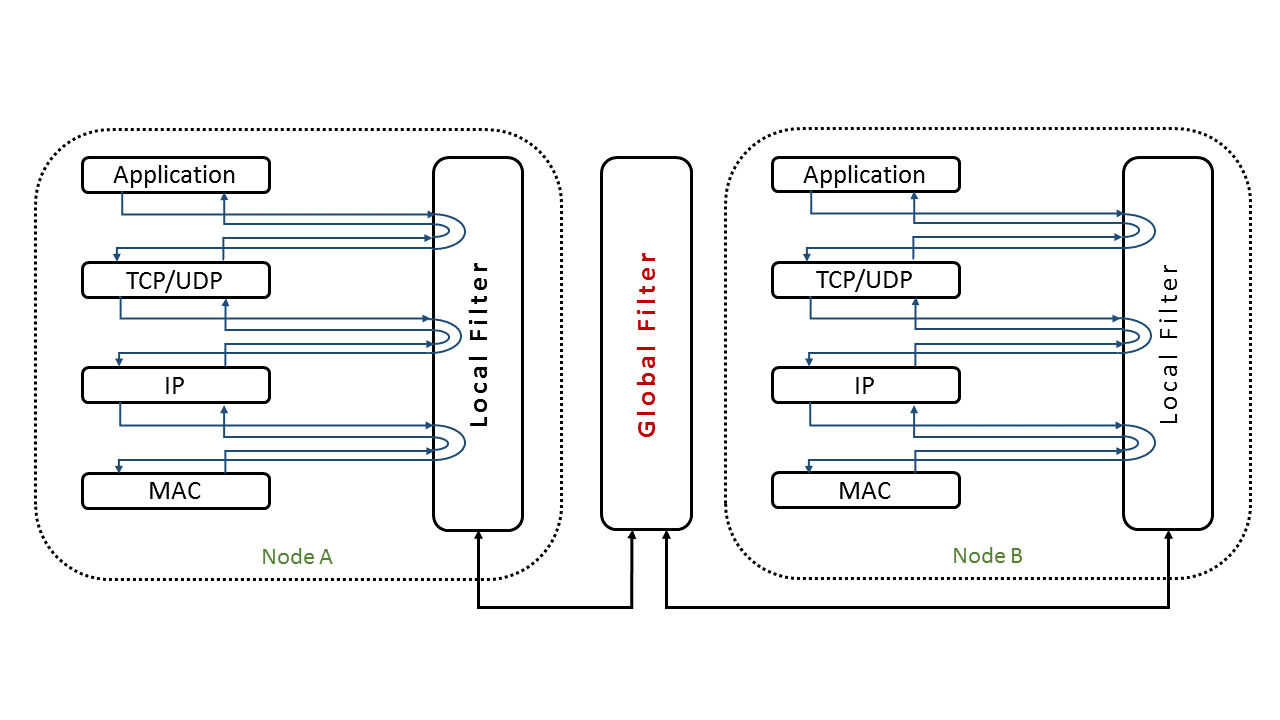
\includegraphics[width=1.2\textwidth]{SEANodes}
\caption{SEA++ Mechanism}
\label{img:seaNodes}
\end{figure}

\texttt{SEA++} has been extended providing support for SDN architectures. The basic mechanism of \texttt{SEA++} has been integrated to OpenFlow switches and SDN controllers and the user is able to describe attack scenarios against these units. This manual describes the ADL primitives of the attack simulator \texttt{SEA++} and shows the steps to run an example either in traditional or SDN networks.
